% Copyright 2013 Aaron Ecay and Meredith Tamminga
% Available under the Creative Commons BY-SA or GPL v2+ licenses: see
% the file LICENSE for more information

\documentclass{digs-slides}
\usepackage{expex}
\usepackage{multicol}
\usepackage{amssymb}
% \bibliographystyle{linquiry2}

\usetikzlibrary{calc}

\newcommand{\includegraph}[2][]{\mode<beamer>{\includegraphics[#1]{#2}}
    \mode<handout>{\includegraphics[#1]{#2-handout}}}

\addbibresource{biblio.bib}

\title{Priming as a diagnostic of grammatical status: Two case studies}
\author{Meredith Tamminga and Aaron Ecay}
\institute{University of Pennsylvania}
\date{Mar.\ 29, 2014 \\\vspace{0.5em} Penn Linguistics Conference 38}

\begin{document}

\begin{frame}
    \titlepage
\end{frame}

\section*{Introduction}

\subsection*{foo}

\begin{frame}{Introduction}
    \begin{itemize}
      \item Diachronic generative syntax encompasses the analysis both
        of historical grammatical structures and of the processes by
        which they change
      \item Analysis of underlying structures is particularly challenging
        without access to native speakers
    \end{itemize}
\end{frame}

\begin{frame}<beamer>
    \frametitle{Introduction}
    \begin{itemize}
      \item Researchers have made headway by using the Constant Rate
        Effect \parencite{Kroch1989} to infer grammatical
        analyses through quantitative data on historical change
      \item We will propose an independent source of quantitative
        evidence about historical grammatical analyses: clustering
        tendencies across tokens
    \end{itemize}
\end{frame}

\begin{frame}
    \frametitle{Table of contents}
    \tableofcontents{}
\end{frame}

\section{Background on priming}

\subsection*{foo}

\begin{frame}{Priming}
    \begin{itemize}
      \item \textbf{Priming:} the tendency to reuse a recently
        encountered linguistic option
      \item Extensive structural priming
        literature \parencite[beginning with][]{Bock:1986}
        demonstrates that syntactic structures can be primed
      \item Example:
        \begin{itemize}
          \item \textbf{Prime:} I gave the children candy
          \item[$\Uparrow$] I gave the dog treats
          \item[$\Downarrow$] I gave treats to the dog
        \end{itemize}
    \end{itemize}
\end{frame}

\begin{frame}{Priming reflects structural identity}
	\begin{itemize}
          \item \textcite{Estival:1985}: different types of passives (lexical vs.\ transformational) each prime themselves but not each other
          \item The structural distinction this reflects is maintained in modern syntactic accounts \parencite[e.g.][]{Embick:2004}
	\end{itemize}
        % Code for this graph:
        % > estival.graph2(write = TRUE)
        \begin{center}
            \includegraph{figures/estival}
        \end{center}
\end{frame}


\begin{frame}{Priming reflects structural identity}
	\begin{itemize}
          \item \textcite{Bock:1990}: Infinitival purpose clauses with
            “to” do not prime prepositional datives with “to”
            \begin{itemize}
              \item I brought a book to study
              \item I brought a book to Stella
            \end{itemize}
          \item \textcite{Ferreira:2003}: complementizer \textit{that}
            presence is not increased by previous use of demonstrative \textit{that}
	\end{itemize}
\end{frame}


\begin{frame}{Priming reflects structural identity}
	\begin{itemize}
		\item Priming can be a useful dependent variable for its reflection of underlying structures: repetition reveals sameness
		\item “If the processing of a stimulus affects the processing of another stimulus, then the two stimuli must be related [...] if the relationship between the two stimuli is syntactic, then we can use this relationship as a way of understanding what syntactic information is represented” \parencite[490]{Branigan:1995}
		\item Linking hypothesis: priming effects in written
                  historical data reflect structural identity in
                  language production at the time
	\end{itemize}
\end{frame}

\section{Case one: Negation}

\subsection{Empirical description}
\label{sec:empirical-aspects}

\begin{frame}{The change in negation}
    \begin{itemize}
      \item In Middle English, there is a change in the exponence of Neg
      \item The negator \emph{ne}, inherited from OE, is lost
      \item \emph{not}, formerly a negative adverb, becomes the new negator
    \end{itemize}
\end{frame}

\begin{frame}{Details of the change}
    \begin{itemize}
      \item During the period of the change, a large number of negative
        sentences have both \emph{ne} and \emph{not}:
    \end{itemize}
    \ex~
    he ne shal nouʒt decieue him \trailingcitation{Early Prose Psalter,
        161:131:11, from \textcite{Frisch1997}}
    \xe
    % To generate this plot:
    % > neg <- cleanNegData("queries/coding.cod.ooo")
    % > three.lines.graph2(neg, write = TRUE)
    \begin{center}
        \includegraph{figures/three-lines2}
    \end{center}
\end{frame}

\subsection{Two analyses}
\label{sec:analyses}

\begin{frame}{Two analyses}
    \begin{multicols}{2}
        \begin{center}
            \textcite{Frisch1997}
            \begin{tikzpicture}[scale=3]
                \node[circle, draw, minimum size=0.6in](ne-atom) at (1,1) {\textsc{ne}};
                \node[circle, draw, minimum size=0.6in](not-atom) at (1,0) {\textsc{not}};
                \node[align=left](ne-surface) at (0,1) {\emph{ne}};
                \node[align=left](ne-not-surface) at (0,0.5) {\emph{ne ... not}};
                \node[align=left](not-surface) at (0,0) {\emph{not}};

                \draw[<-,>=triangle 45] (ne-atom) -- (ne-surface);
                \draw[<-,>=triangle 45] (ne-atom) -- (ne-not-surface);
                \draw[<-,>=triangle 45] (not-atom) -- (not-surface);
                \draw[<-,>=triangle 45] (not-atom) -- (ne-not-surface);
            \end{tikzpicture}
        \end{center}

        \begin{center}
            \textcite{wallage08}
            \begin{tikzpicture}[scale=3]
                \node[circle, draw, minimum size=0.55in](ne-atom) at (1,1) {\textsc{ne}};
                \node[circle, draw, minimum size=0.55in](ne-not-atom) at (1,0.5) {\textsc{ne-not}};
                \node[circle, draw, minimum size=0.55in](not-atom) at (1,0) {\textsc{not}};
                \node[align=left](ne-surface) at (0,1) {\emph{ne}};
                \node[align=left](ne-not-surface) at (0,0.5) {\emph{ne ... not}};
                \node[align=left](not-surface) at (0,0) {\emph{not}};

                \draw[<-,>=triangle 45] (ne-atom) -- (ne-surface);
                \draw[<-,>=triangle 45] (ne-not-atom) -- (ne-not-surface);
                \draw[<-,>=triangle 45] (not-atom) -- (not-surface);
            \end{tikzpicture}
        \end{center}
    \end{multicols}
\end{frame}

\begin{frame}
    \frametitle{Results (PPCME2)}
    \begin{multicols}{2}
        % > nnb.fac.graph2(neg, write = TRUE)
        \includegraph[width=\linewidth]{figures/ne-not2}
        % > patch.graph2(neg, write = TRUE)
        \includegraph[width=\linewidth]{figures/patch2}
    \end{multicols}
\end{frame}

\section{Case two: \emph{do}-support}
\label{sec:case-two:-emphdo}

\subsection{Empirical description}
\label{sec:empir-descr}

\begin{frame}
    \frametitle{\emph{Do}-support}
    \begin{itemize}
      \item In the Early Modern English (EME) period (1500–1700),
        the use of auxiliary \emph{do} became obligatory in English
        negative declaratives and questions (inter alia)
      \item During the course of this change there was a period when
        \emph{do} was used in (non-emphatic) affirmative declaratives,
        which is banned in present-day English
    \end{itemize}
    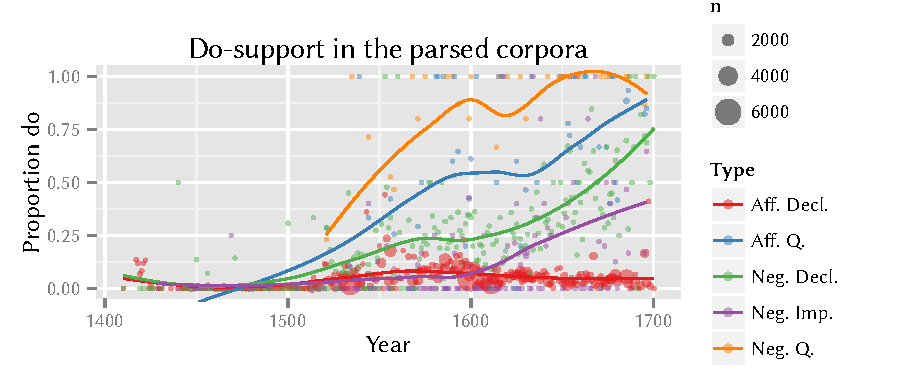
\includegraphics[width=\textwidth]{static-figures/do-all}
\end{frame}

\begin{frame}
    \frametitle{Two kinds of \emph{do}}
    \begin{itemize}
      \item \textcite{Ecay2012a} proposed that the \emph{do} found in
        affirmative declaratives is distinct from the modern type of
        \emph{do}, is merged lower than T, and functions in early EME as
        a marker of argument structure
    \end{itemize}
    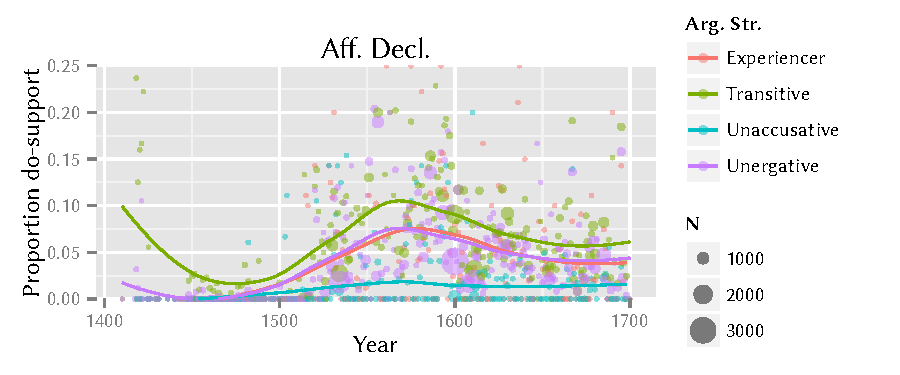
\includegraphics[width=\textwidth]{static-figures/do-aff}
    \begin{itemize}
      \item If this is so, it should be visible in priming data
    \end{itemize}
\end{frame}

\subsection{Predictions}
\label{sec:predictions}

\begin{frame}
    \frametitle{Priming predictions for \emph{do}}
    \begin{itemize}
      \item The intermediate (low-\emph{do}) grammar can produce surface
        \emph{do} in affirmative declarative contexts
      \item It can \textbf{also} do so in modern \emph{do}-support
        contexts (with external argument)
      \item The modern (high-\emph{do}) grammar can produce surface
        \emph{do} only in the modern \emph{do}-support contexts
      % \item Thus, three types of grammatical objects: affirmative
      %   declarative produced by intermediate grammar, modern-type do
      %   produced by intermediate grammar, and modern-type do produced by
      %   modern grammar
    \end{itemize}
\end{frame}

\begin{frame}
    \begin{center}
        \begin{tikzpicture}[xscale=1.55]
            \node[circle,draw,minimum size=0.75in] (v1) at (-3.5,4.5) {Intermed.};
            \node[circle,draw,minimum size=0.75in] (v2) at (0.5,4.5) {Intermed.};

            \node[circle,draw,minimum size=0.75in,visible on=<2>] (v4) at (-3.5,2) {Intermed.};
            \node[circle,draw,minimum size=0.75in,visible on=<2>] (v3) at (0.5,2) {Intermed.};

            \node[circle,draw,minimum size=0.75in] (v5) at (-3.5,-0.5) {Modern};
            \node[circle,draw,minimum size=0.75in] (v6) at (0.5,-0.5) {Modern};

            \draw ($(v4.north west)+(-0.1in,0.15in)$) rectangle ($(v5.south east)+(0.1in,-0.15in)$);
            \draw ($(v3.north west)+(-0.1in,0.15in)$) rectangle ($(v6.south east)+(0.1in,-0.15in)$);
            \draw ($(v2.north west)+(-0.1in,0.15in)$) rectangle ($(v2.south east)+(0.1in,-0.15in)$);
            \draw ($(v1.north west)+(-0.1in,0.15in)$) rectangle ($(v1.south east)+(0.1in,-0.15in)$);

            \node[draw] at (-1.5,5) {Affirmative declarative};
            \node[draw] at (-1.5,0.5) {Modern contexts};
            \draw [->,>=triangle 45] (v1) edge (v2);
            \draw [->,>=triangle 45,visible on=<2>] (v1) edge (v3);
            \draw [->,>=triangle 45,visible on=<2>] (v4) edge (v2);
            \draw [->,>=triangle 45,visible on=<2>] (v4) edge (v3);
            \draw [->,>=triangle 45] (v5) edge (v6);

            \node at (-3.5,6) {\textbf{Prime}};
            \node at (0.5,6) {\textbf{Target}};
        \end{tikzpicture}
    \end{center}
\end{frame}

\subsection{Results}
\label{sec:results}

\begin{frame}
    \frametitle{Results}
    % > source("scripts/dosupp.R")
    \includegraph[width=\textwidth]{figures/do-results}
\end{frame}

\begin{frame}<handout>
    \frametitle{Results (PPCEME + PCEEC)}
    \begin{itemize}
      \item Affirmative declaratives always prime each other, as expected
      \item Modern environments prime each other more strongly over
        time, as disguised affirmative declaratives disappear
      \item Cross-priming lessens over time, also related to the
        disappearance of disguised affirmative declaratives
    \end{itemize}
\end{frame}

\section{Conclusions}
\label{sec:conclusion}

\subsection*{foo}

\begin{frame}{Conclusions}
    \begin{itemize}
      \item The Constant Rate Effect is important because it
        provides a link between frequency data attested in historical
        corpora and the mental representations that underlie language
        and language change
      \item We would like to suggest that priming data constitute
        another, independent source of linkage between these two domains
        \begin{itemize}
          \item As has been shown in our two case studies
        \end{itemize}
      \item The investigation of priming evidence can support and refine
        the conclusions of quantitative studies of syntactic change
    \end{itemize}
\end{frame}

\begin{frame}
    \frametitle{Conclusions}
    \begin{itemize}
      \item Priming research has been deployed in studies of spoken
        corpora to answer questions about grammatical variation in
        contemporary American English and Romance languages
      \item There is also a large and growing experimental literature on
        structural priming, to which this work creates obvious bridges
      \item We would love to see more linguists using priming methods as
        a tool to understand their favorite variables!
    \end{itemize}
\end{frame}

\appendix{}

\section{Acknowledgments}

\subsection{foo}

\begin{frame}
    \frametitle{Acknowledgments}
    We would like to thank the following:
    \begin{itemize}
      \item The compilers of the corpora used (PPCME2, PPCEME, PCEEC)
      \item Beatrice Santorini
      \item Tony Kroch
      \item Our fellow graduate students at Penn
      \item The audience of DiGS15 for comments on an earlier version
        (containing the negation results)
    \end{itemize}
\end{frame}

\begin{frame}
    \frametitle{High technology}
    All the data and code used in this analysis is available on GitHub:
    \url{https://github.com/aecay/digs15-negative-priming}
    \mode<beamer>{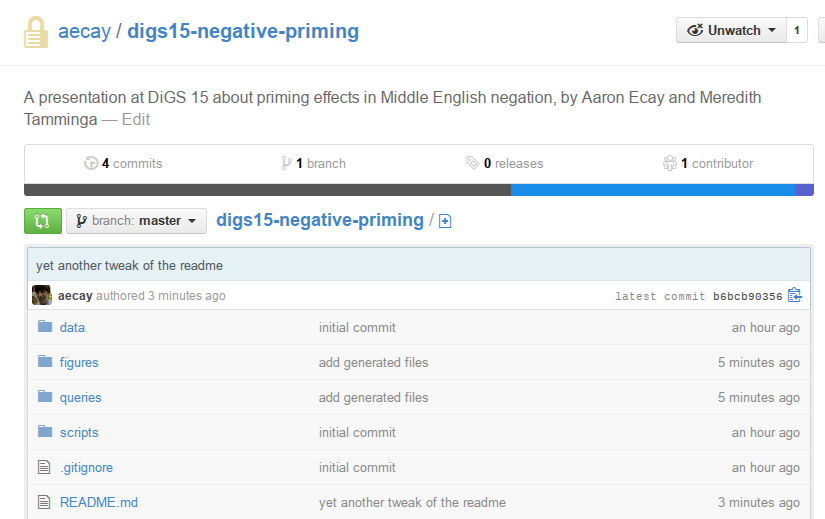
\includegraphics[height=3in]{figures/github}}
\end{frame}

\begin{frame}<beamer>
    \frametitle{Questions}
    \begin{center}
        \Huge
        Questions?
    \end{center}
\end{frame}

\section{Bibliography}
\label{sec:bibliography}

\subsection*{foo}

\begin{frame}[allowframebreaks=0.9]{Bibliography}
    \printbibliography[heading=none]
\end{frame}

% TODO: put details about the negation patch in bonus slides section


\end{document}
